\documentclass[letterpaper]{article}

\usepackage{aaai}
\usepackage{amsmath}
\usepackage{amssymb}
\usepackage{amsthm}
\usepackage{courier}
\usepackage{graphicx}
\usepackage{helvet}
\usepackage{hyperref}
\usepackage{times}
\usepackage{verbatim}

\newtheorem{definition}{Definition}
\newtheorem{example}{Example}
\newtheorem{formula}{Formula}
\newtheorem{problem}{Problem}

%\setlength\parindent{0pt}
\frenchspacing

\setlength{\pdfpagewidth}{8.5in}
\setlength{\pdfpageheight}{11in}

\pdfinfo{
/Title Rough Set Semantics for Identity Management on the Web
/Author Wouter Beek, Stefan Schlobach, Frank van Harmelen}
\setcounter{secnumdepth}{0}

\begin{document}

\title{Rough Set Semantics for Identity Management on the Web}
\author{Wouter Beek \and Stefan Schlobach \and Frank van Harmelen\\
Vrije Universiteit Amsterdam\\
De Boelelaan 1081a\\
1081HV Amsterdam\\
The Netherlands}
\maketitle
\begin{abstract}
\begin{quote}
Identity relations are at the foundation of the Linked Open Data initiative and on the Semantic Web in general. They allow the interlinking of alternative descriptions of the same thing. However, many practical uses of \verb|owl:sameAs| are known to violate its formal semantics. We propose a method that treats a given identity relation as a partition of collections of indiscernability pairs, assigning meaning to identity subrelations in terms of predicates in the schema of the dataset. Reinterpreting identity in this way allows the calculation of a higher and lower approximation, creating a rough set description of identity. SOMETHINGSOMETHING
\end{quote}
\end{abstract}

\section{Introduction}
\label{sec:introduction}

Identity relations are at the foundation of the Linked Open Data initiative and of the Semantic Web in general \cite{bizer_cyganiak_heath_2007}. They allow the interlinking of alternative descriptions of the same thing. However, the traditional notion of identity (expressed by \verb|owl:sameAs| \cite{motic_paterschneider_grau_2012}) is often problematic, e.g. when objects are considered the same in some contexts but not in others. The standing practice in such cases is to use weaker relations of relatedness (e.g. \verb|skos:related|). Unfortunately, this limits reasoners in drawing inferences.

According to the traditional semantics of the identity relation, identical terms can be replaced for one another in all non-modal contexts \emph{salva veritate}. Practical uses of \verb|owl:sameAs| are known to violate this strict semantics \cite{halpin_hayes_2010,halpin_hayes_mccusker_mcguinness_thompson_2010}.

\subsection{Previous work}
\label{sec:previous_work}

Existing research proposes the following solutions for the problem of identity relations in the Semantic Web. (1) Introduce weaker versions of \verb|owl:sameAs| \cite{halpin_hayes_2010,mccusker_mcguinness_2010} (e.g., \verb|skos:related|). (2) Restrict the applicability of identity relations to specific contexts. Identies are expected to hold with a named graphs or within a namespaces, but not necessarily outside of it \cite{halpin_hayes_2010,melo_2013}. (3) Introduce additional vocabulary that does not weaken but extend the existing identity relation \cite{halpin_hayes_2010}. For example, allow an explicit distinction to be made between mentioning a term and using a term (e.g. a car and a Web document describing that car). (4) Add domain-specific weaker versions of the identity relation \cite{mccusker_mcguinness_2010} (e.g., ``have the same medical use'' is weaker than ``are the same molecure''). (5) Adapt the modeling practice, possibly in a (semi-)automated way by adapting visualization and modeling toolkits to produce notifications upon reading data. This can for example be done by giving a warning upon importing an identity pair from an external resourse. Alternatively, additional restrictions can be put on changing and creating data. For example adding an RDF link could require reciprocal confirmation from the maintainers of the respective datasets. \cite{halpin_hayes_2010,ding_shinavier_finin_mcguinness_2010}

Other related research focusses on the extraction of network properties of \verb|owl:sameAs| datasets \cite{ding_shinavier_shangguan_mcguinness_2010}, but these endeauvours are not yet related to the semantics of the identity relation.

What these approaches have is common is that quite some work has to be done (adapting or creating standards, instructing modelers, converting existing dataset) in order to resolve some of the problems of identity. Our approach provides a way of dealing with the heterogenous real-world usage of identity in the Semantic Web that is fully automated and that requires no changes to standards, modeling practices, or existing datasets.

\subsection{Research goals}
\label{sec:research_goals}

In developing our new approach we have the following research goals:

\begin{enumerate}
\item In an identity relation the pairs all look the same. We want to characterize subrelations in terms of the predicates that occur in the schema of the dataset. In this way we can distinguish between different types of identity by assigning meanings to sets of indentity pairs.
\item Based on an exiting identity relation, and using concepts from rough set theory, we can define an approximation of that identity relation. Based on the approximation, semantically moticated suggestions can be given for extending and/or limiting the identity relation.
\item The quality of an identity relation can be characterized in terms of the accuracy of the rough set approximation.
\end{enumerate}

\section{Approach}
\label{sec:approach}

In the following we shall consider an arbitrary graph $G$. The resources (excluding blank nodes) that occur as the subject term of some triple in $G$ are called $S_G$. We choose not to include blank nodes in our approach, since identity relations are almost never defined between them. The resources that occur as the predicate term of some triples in $G$ are called $P_G$. In the following we assume that $G$ is a fully materialized graph.

For illustrative purposes we shall use the IIMB dataset as it is used in the instance matching track of the Ontology Alignment Evaluation Initative 2012 \cite{oaei_2012}. This dataset consists of eighty ontologies that are linked to a single base ontology. For each of these eighty links a reference mapping is available. The graphs $G$ are the result of merging the two linked graphs.

We will use the words `property' and `predicate' in order to denote sligtly different things. A \emph{property} is taken to be a predicate-object pair. Examples of properties are ``is spoken in Germany'' and ``has a democratic form of government''. Examples of \emph{predicates} are ``is spoken in'' and ``form of government is''.

In theory it is possible to construct properties of arbitrary depth (in terms of the distance to the subject term) by using blank nodes to existentially quantify over intermittent resources. For example ``is spoken in a country with a democratic form of government'' is a property that quantifies over countries and that may be shared by the languages French and Dutch. In this paper we only consider properties of `depth one', i.e. properties that consits of a single predicate and object term.

\subsection{Shared properties and indiscernability}
\label{sec:indiscernibility}

When we look at the triples that constitute a set of identity relations, we see that all links look the same. But when we take the triples in which the subject and object terms occur into account, we see that within the identity relation there may be different subrelations that we can identify in terms of the predicates that occur in the schema.

For instance, in the IIMB graphs there are some identical resources that share the property \verb|IIMBTBOX:spoken_in|, while other pairs share the property \verb|IIMBTBOX:form_of_government|. The set of pairs of resources that are spoken in the same language may even be disjoint from the set of pairs of resources that have the same form of government.

Note that we are not only interested in the properties that resources share with one other (e.g., where they are spoken, or which form of government they have), but we are also interested in resource pairs that share the same sharing properties. We can thus identify subsets of an identity relation based on differences in the sets of predicates relative to which they take resources to be \emph{indiscernable} from one another.

In the example above, one subset of the identity relation does not discern resources that are spoken in the same language, whereas another subset of the identity relation does not discern resources that have the same form of government.

As in rough set theory, we define indiscernability as a set of pairs for which it is impossible to show the distinction. We therefore say that two resources are indiscernible with respect to a set of predicates $P$ ($IND(P)$, definition \ref{def:unary_indiscernability}) in case they share the same properties. We say that two resource pairs are indiscernible ($IND(P^*)$, definition \ref{def:binary_indiscernability}) in case both pairs are indiscernible for the same $P^* \subseteq \mathcal{P}(P_G)$.

\begin{definition}[Indiscernability]
\begin{align}
IND(P) = \{
  \langle x, y \rangle \in S_G^2
\  \vert \ 
  \forall a \in P(a(x) = a(y))
\}
\label{def:unary_indiscernability}
\\
IND(P^*) \  = \  \{
    \langle
      \langle x_1, y_1 \rangle,
      \langle x_2, y_2 \rangle
    \rangle \in (S(G)^2)^2
  \  \vert \ 
\nonumber
\\
    \forall P \in P^*(P(x_1, y_1) = P(x_2, y_2))
  \}
\label{def:binary_indiscernability}
\end{align}
\end{definition}

As explained above, for a given set of identity pairs there may be multiple pairs that have the same shared properties. These sets of predicates that are shared across resource pairs are considered to give a description of a specific subrelation of the identity relation. For example, in figure \ref{fig:indiscernibility_example} the subrelation $\{ \langle a, c \rangle, \langle b, c \rangle \}$ is characterized by $\mathcal{P}(\{ P \})$.

\begin{figure}
\caption{This figure contains four resources, represented by nodes and annotated with the properties $P$, $Q$, and $R$ that apply to them. It also contains six pairs, represented as edges between the nodes (reflexive pairs are not shown). The edges are drawn inside squares that represent the indiscernability sets to which they belong. For instance $\langle a, c \rangle$ and $\langle a, c \rangle$ belong to the same indiscernability set $\{ P \}$, but $\langle a, b \rangle$ belongs to indiscernability set $\{P, Q\}$.}
\label{fig:indiscernibility_example}
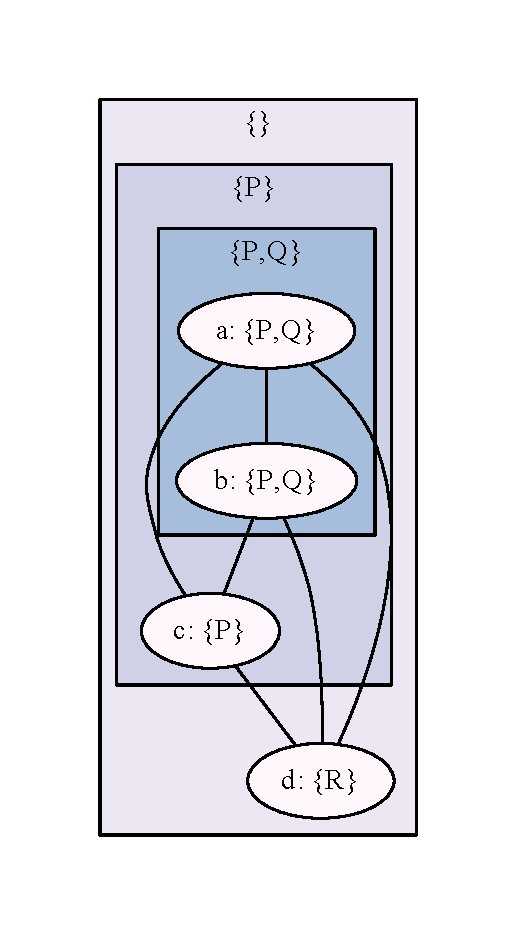
\includegraphics{indiscernibility_example}
\end{figure}

According to the standard definition, identical resources are indiscernable with respect to all properties. We take a given set of identity pairs and partition it into subsets which we can describe as being $P$-indiscernable, for $P \subseteq P_G$.

REDO THIS FUGIRE WITH LESS DETAIL.
Figure \ref{fig:indiscernability_iimb} shows the partitioning of the indentity relation of IIMB dataset number 22.

\begin{figure}
\label{fig:indiscernability_iimb}
\caption{The partition of the identity relation of IIMB dataset number 21. For each partition we give the number of identity pairs that belong to the partition. For instance, there are XXX identity pairs that are $\{ YYY \}$-indiscernable, while there are ZZZ identity pairs in total.}
\includegraphics[scale=0.5]{iimb_21}
\end{figure}

\section{Approximation}
\label{sec:approximation}

In the previous section we partitioned a given identity relation in subrelations that can be distinguished in semantic terms (i.e., subsets of $P_G$). In this section we create an approximation of the identity relation. This approximation will allow us to (1) quantify the quality of the linkset, and (2) give suggestions about which pairs to include in / exclude from the identity relation.

For the approximation of the identity relation we use rough set theory [REF] to represent an approximation of a given identity relation called $\approx$. The domain for our rough set approach is the Cartesian product of $S_G$. The set of predicates is the powerset of $P_G$.\footnote{Relations are called attributes in rough set theory, and they are functions that map to an arbitrary set of value labels. We only consider functions that map from binary input onto the set of Boolean truth values, and therefore call these `predicates'.} This means that we have a big number of primitives to work with (quadratic in the number of constants; exponential in the number of relations).

For an arbitrary binary relation $\approx$ we can define a higher ($\overline{\approx}$, definition \ref{def:higher_approximation}) and a lower ($\underline{\approx}$, definition \ref{def:lower_approximation}) approximation of that relation, where $\mathbb{R}$ characterizes a similarity relation between resource pairs. The intuition behind these definitions is that non-$approx$-pairs that are similar to $\approx$-pairs should be in the higher approximation, whereas no $\approx$-pair that has a similar non-$\approx$-pair should be in the lower approximation.

\begin{definition}[Higher \& lower approximation]
\begin{align}
x \overline{\approx} y \  & \iff & \ 
  \exists u,v (
      \mathbb{R}(\langle u, v \rangle, \langle x, y \rangle)
    \land
      u \approx v
  )
\label{def:higher_approximation}
\\
x \underline{\approx} y \  & \iff & \ 
  \forall u,v (
      \mathbb{R}(\langle u, v \rangle, \langle x, y \rangle)
    \rightarrow
      u \approx v
  )
\label{def:lower_approximation}
\end{align}
\end{definition}

\begin{comment}
\begin{definition}[Higher \& lower approximation]
\label{def:higher_lower_approximation}
\begin{align}
y \in [x]_H \  \text{iff} \  \exists [u]_{\approx} (
    \vert [u]_{\approx} \vert > 1
  \land
    \mathbb{P}([u]_{\approx}) = \mathbb{P}(\{ x, y \})
  ) \\
y \in [x]_L \  \text{iff} \  \forall S \subseteq D (
    (\vert S \vert > 1 \land \mathbb{P}(S) = \mathbb{P}(\{ x, y \}))
  \rightarrow
    \exists s \in D (S = [s]_{\approx})
  )
\end{align}
\end{definition}
\end{comment}

Since we want to stay close to the traditional notion of identity, defined in terms of indiscernability, we choose $IND(\mathcal{P}(P_G))$, defined in \ref{def:binary_indiscernability}, as our $R$.

Figure \ref{fig:approximation_iimb} shows the lower and higher approximations for the 22th IIMB ontology alignment (see figure \ref{fig:indiscernability_iimb}). Since a partition is only drawn when there is at least one identity pair that is indiscernable with respect to some set of predicates, the higher approximation amount to the entire figure. The lower approximation only consists of those partition sets for which the number of identity pairs is the same as the number of pairs.

\begin{figure}
\label{fig:approximation_iimb}
\caption{The discernability partition of the identity relation of IIMB alignment 21, plus its lower and higher approximation.}
\includegraphics[scale=0.5]{iimb_21}
\end{figure}

\subsection{Quality}

Given the rough set representation $\langle \underline{\approx}, \overline{\approx} \rangle$ of identity relation $\approx$, we can calculate the accuracy of this approximation with equation \ref{eq:accuracy}.

\begin{equation}
\label{eq:accuracy}
\alpha_P(\approx) = \frac{\vert \underline{\approx} \vert}{\vert \overline{\approx} \vert}
\end{equation}

The rough set approximation accuracy provides a metric for linkset quality.

\section{Evaluation}
\label{sec:evaluation}

\subsection{Implementation}
\label{sec:implementation}

The implementation that was built for this paper is deployed as a CPACK (extension pack) of the ClioPatria triple store \cite{schreiber_2006}. For RDF graphs that are loaded in ClioPatria this extension can calculate the discernability partition and rough set approximation and accuracy. The results are displayed as an SVG graph. Interactive Ajax code allows the user to click on paratition sets of the SVG graph to navigate to a description of the resource pairs that $P$-indiscernable but that are not in the identity relation (see figure \ref{fig:screenshot}).

\begin{figure}
\label{fig:screenshot}
\caption{Screenshot of the SVG graph and the tabular description of non-identity pars that are $P$-indiscernable. The tabular view groups the overlapping and disjoint properties of two resources.}
%\graphics{}
\end{figure}

\subsection{Hypotheses}
\label{sec:hypotheses}

We use the indiscernability partition of an identity ralation, its lower and higher approximations, and its accuracy, in order to validate the following hypotheses.

The quality of a linkset is correlated with the accuracy metric.

\section{Conclusion}
\label{sec:conclusion}

Reflexivity, symmetry and (in some cases) transitivity are preserved under indiscernability, allowing reasoners to infer new results.

In this paper we have defined (1) the indiscernability partition of an identity ralation, (2) its lower and higher approximations, and (3) its accuracy.

(1) allows an identity relation to be divided up into subrelations with a different meaning. The meaning is expressed in domain-dependent terms, drawing predicates from the schema of the dataset.

Based on (2) it is possible to identify pairs for inclusion in / exclusion from the identity relation. Together with (3) this provides a way of establishing the quality of the subrelations identifies in (1), or the identity relation as a whole.

We think that these qualitative means of characterizing an identity relation are a useful addition to existing quantitative means. Also, we think that it is more useful and viable to enrich existing identity relations in the LOD based on the semantics of the graphs in which they occur, than to introduce new relationships into Semantic Web languages to which modelers should conform. Appart from the practical difficulties of teaching practitioners and transforming/enriching existing datasets, we may claim that the exact meaning of an identity (sub)relation is only defined in its use, i.e., in the indiscernability criteria it embodies.

We are currently in the process of validating the hypotheses enumerated in the previous section. The results of these evaluations are continuously published on \url{https://wouter-beek.squarespace.com/identity-on-the-web/}. The website currently contains the automated results of all 80 IIMB alignments. The website also refers to the publicly available Git repository \url{https://github.com/wouterbeek/IOTW} where the implementation discussed in section \ref{sec:implementation} can be found.

For our approach it is not necessary to pose additional restrictions on the binary relation. In practice this will be either a linkset relating subgraphs of $G$ to each other, or a set of alignments created by an ontology mapping tool.

\footnote{A linkset is a collection of RDF links. An RDF link is an RDF triples whose subject and object terms are described in different datasets. \cite{void_2011} The predicate term of an RDF link is often the identity relation.}

\bibliographystyle{aaai}
\bibliography{rough_set_semantics_for_identity_management_on_the_web}

\end{document}

